
\newpage
\section{Machine Learning}
\subsection{Definition and Overview}
By definition, machine learning is the process by which a computer is able to improve its own performance (as in analyzing image files) by continuously incorporating new data into an existing statistical model. 

It can also be defined as "the branch of computer science dealing with the creation and use of computer software that employs machine learning" \parencite{mw:machine-learning}.

However, researchs have a differing opinion on the definition. One has defined machine learning as a branch of computational algorithms that emulate human intelligence by learning from the environment \parencite{ElNaqa2015}, while another describes machine learning as a study of computational methods for improving performance by mechanizing the acquisition of knowledge from experience \parencite{Langley1995}. 

Besides that, machine learning has also been described as a way to address problems where phenomena are changing rapidly, or where applications need to be customized for each user separately \parencite{Dietterich1996}.

Commonly, ML is classified into supervised, unsupervised, and reinforcement learning. However, there can also be semi-supervised, transduction and learning to learn algorithms \parencite{Oladipupo2010}. 

Supervised learning is typically used for prediction tasks, where a model is trained using labeled data. 

Unsupervised learning involves finding hidden patterns or intrinsic structures from unlabeled data. Reinforcement learning enables a software agent to learn in an interactive environment by trial and error.

Within the broader machine learning landscape, a particularly noteworthy development is the emergence of deep learning. Deep learning is described as a network of nodes and edges that resemble the biological communication of brain neurons \parencite{Dinov2018}. 

Deep learning algorithms, often based on neural networks, can model high-level abstractions in data, thereby providing enhanced predictive accuracy in tasks such as image and speech recognition, natural language processing, and more.

\newpage
\subsection{Applications}
Machine learning's potential for pattern recognition and predictive analysis has led to a broad array of applications across multiple domains. This includes cyber security, healthcare, and intelligent transportation systems, to name a few. \parencite{Jhaveri2022}.

Socially, ML has made a big impact too. Social media has utilised machine learning to analyze large amounts of data, where for example Twitter, where it has been used to identify real and fake tweets \parencite{Arora2018}.

The reality is, machine learning is almost applied everywhere. A mobile phone is now capable of web search, online advertising, product recommendations, object recognition, intelligent control, decision making, speech recognition, natural language processing, computer graphics, and computer vision, which is all powered by machine learning itself. As time goes on, the importance keeps getting even more significant as it slowly integrates to everyone's daily lives.\\

\newpage
\subsection{Machine Learning in Healthcare}
Healthcare stands out as a domain particularly poised to benefit from the advancements in machine learning. machine learning has been applied in a lot of areas, including medical imaging, natural language processing of medical documents, genetic information, disease prediction, disease detection, and personalized healthcare \parencite{Mana2022}.

Another key applications of ML in healthcare is in the field of medical imaging. In terms of radiology, it has shown that machine learning has potential to improve various aspects of radiology, including detection and interpretation of findings, postprocessing, and radiology reporting \parencite{Choy2018, Erickson2017}.

Another significant area of application is in predictive healthcare. machine learning algorithms Naïve Bayes, Decision Tree, Random Forest, and K-Nearest Neighbors are being utilised to predict diseases based on symptoms and large datasets of medical procedures \parencite{Garg2023}.\\

\newpage
\subsection{Feature Extraction and Selection}
Feature extraction and selection are crucial processes in any machine learning model. They involve identifying and selecting the most relevant information from raw data to be used for machine learning.

In the context of healthcare, feature extraction and selection could be applied to a variety of data, such as medical imaging, genomic data, or patient records. For instance, in Magnetic Resonance Imaging (MRI) feature extraction approach utilizes spatial filters, edge detection algorithms, and wavelet transform-based image fusion \parencite{Udomhunsakul}.

In handwriting analysis, features could refer to the stroke width, stroke length, speed, pressure, and slant among others. These characteristics can be critical in distinguishing between dyslexic and non-dyslexic handwriting. Selecting the right features is crucial as it directly impacts the performance of the machine learning model \parencite{Arif2015}.\\

\newpage
\subsection{Machine Learning Algorithms}
Machine learning algorithms are the crux of any ML model, determining how it learns from data and makes predictions or decisions. The choice of algorithm often depends on the nature of the task and the data at hand, with a wide range of algorithms available each with unique strengths and limitations.

Some of machine learning algorithms include K-Nearest Neighbors, Naïve Bayes, Support Vector Machine, Decision Tree, and others. These have been widely used in various fields, including healthcare, due to their interpretability and robustness \parencite{Ray2019}.

In recent years, deep learning algorithms, such as convolutional neural network and recurrent neural network, have gained popularity. These algorithms can learn complex patterns in data, making them highly effective for tasks that involve large amounts of data or that require the extraction of intricate features \parencite{Pamina2019SurveyOD}.\\

\newpage
\subsection{Performance Evaluation}
Evaluating the performance of machine learning models is essential to verify their effectiveness and reliability. Metrics such as accuracy, precision, recall, and F1 score are commonly used for this purpose. However, the choice of metrics should align with the problem at hand, as different tasks may require prioritizing different aspects of the model's performance.

In addition to these metrics, consideration of the model's robustness against variations in the data is crucial. This could involve testing the model under different conditions, or using different subsets of the data, to ensure that it performs consistently and does not overly rely on specific characteristics of the training data. 

There are a bunch of methods to evaluate robustness, including prediction consistency between source and target data in the neighborhood of the source samples \parencite{Shi2019} and a framework for evaluating robustness to changes in setting or population using a single, fixed evaluation dataset \parencite{Subbaswamy2020EvaluatingMR}.

Another important aspect of performance evaluation is the interpretability of the model. While some complex models, like deep learning models, may achieve high performance, they are often regarded as 'black boxes' due to their lack of interpretability \parencite{Zhang2018}. On the other hand, simpler models may offer more interpretability, but at the cost of performance. Striking a balance between these factors is an ongoing challenge in the field of machine learning.\\

\newpage
\subsection{Limitations and Challenges}
Despite the promising advancements, machine learning is not without its challenges and limitations. The quality and diversity of data is one of the primary concerns. machine learning models thrive on large amounts of high-quality, representative data. However, in situations where data is scarce, imbalanced, or inherently biased, the model's performance may be compromised \parencite{Lum2017}.

Another concern is overfitting, where the model learns the training data too well, to the point that it performs poorly on unseen data \parencite{Ying2019}. This issue highlights the importance of proper model validation and testing methodologies.

Data privacy is a crucial challenge across many domains that use machine learning. Ensuring the protection and appropriate use of sensitive data is a complex issue that often requires navigating regulatory and ethical considerations \parencite{Strobel2022}.\\

\newpage
\section{Artificial Neural Network (ANN)}
\begin{figure}[h]
    \centering
    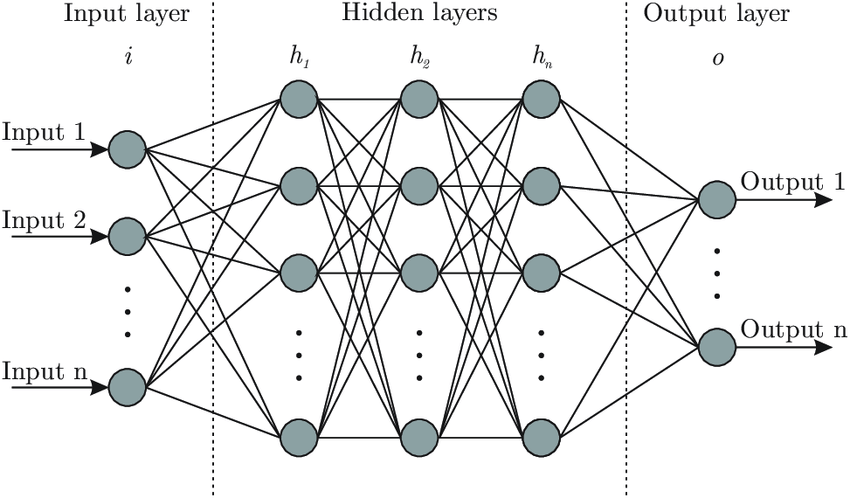
\includegraphics[scale=0.4]{images/literature review/ANN.png}
    \caption{Artificial Neural Network architecture}
    \label{fig:ANN}
    \parencite{Bre2017}
\end{figure}
Artificial neural network (ANN) are a mathematical model that simulates the structure and functionalities of biological neural networks. ANNs are composed of interconnected processing elements (neurons) that work together to solve specific problems. ANNslearn by example and are configured for specific applications, such as pattern recognition or data classification, through a learning process. ANNs have the ability to extract patterns and detect trends that are too complex for humans or other computer techniques to notice \parencite{Krenker2011}.

ANNs have remarkable ability to derive meaning from complicated or imprecise data, can be used to extract patterns and detect trends that are too complex to be noticed by either humans or other computer techniques \parencite{Zakaria2014ArtificialNN}.

At the simplest level, an ANN consists of nodes (or 'neurons') connected by 'synapses', which transmit signals between the nodes. The strength of these connections, or weights, are adjusted during training, allowing the network to learn from the input data \parencite{Sonali2014ResearchPO}.

ANNs have proven effective across a range of tasks, from image and speech recognition to natural language processing. One of their key strengths is their ability to learn and model non-linear and complex relationships, which makes them particularly useful in scenarios where the relationship between input and output is unknown or hard to define. 

These applications include the use of ANNs in predicting properties of concrete-like composite materials \parencite{Kasperkiewicz2000}, to solve differential equations in radio frequency (RF) engineering \parencite{Pattanaik2008}, and in food science, including modeling microbial growth, interpreting spectroscopic data, and predicting physical, chemical, functional, and sensory properties of food products \parencite{Huang2007}. 

However, despite its strengths, ANNs also have their challenges. One claims that it has two main limitations, which are over-training and its inability to extrapolate beyond the range of existing data \parencite{Yin2003}. Other than that, ANNs have difficulty of realizing non-linear sigmoidal activation functions \parencite{Mitra2016}.


\newpage
\section{Convolutional Neural Network (CNN)}
\begin{figure}[h]
    \centering
    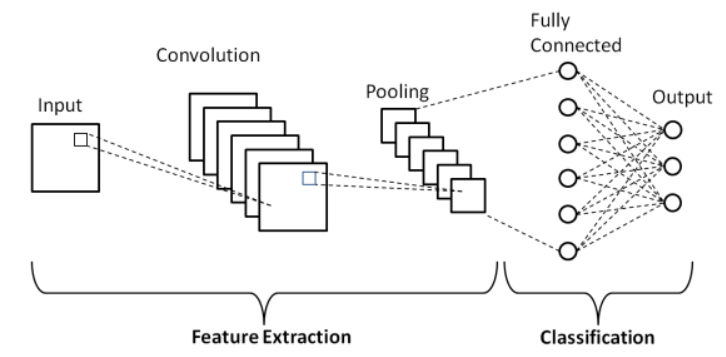
\includegraphics[scale=0.7]{images/literature review/CNN.png}
    \caption{Convolutional Neural Network architecture}
    \label{fig:CNN}
    \parencite{Phung2019}
\end{figure}
Convolutional neural network (CNN) are a type of artificial neural network specifically designed for processing data with a grid-like topology, such as images. They have demonstrated impressive successes in applications such as computer vision for tasks such as face recognition, scene labeling, image classification, and natural language processing for speech recognition and text classification. \parencite{Bhandare2016ApplicationsOC} \parencite{TaiyabaAnsari2022}.

The architecture of CNN is designed to mimic the way a human eye focuses on objects. It consists of one or more convolutional layers, often followed by pooling layers, fully connected layers, and normalization layers. The convolutional layer performs a convolution operation that focuses on small squares of input data, preserving spatial relationships between pixels \parencite{Purwono2023}.

One distinctive feature of CNNs is the use of a technique known as 'weight sharing' in their convolutional layers, where the same filter (weights) is used for each part of the input. This allows the network to learn features that are useful across the entire image, reducing the number of parameters in the model, and thereby reducing overfitting.

Despite their effectiveness, CNNs also have their challenges. They require substantial computational resources, making them expensive to train. Not just that, they lack true understanding and may make obvious mistakes, especially during deliberate testing rounds or on samples outside the training distributions \parencite{Yan2017HowIA}. 

Furthermore, they require large amounts of labeled data, which may not always be available. CNNs are also susceptible to adversarial attacks, wherein small, purposely designed changes to input can lead the network to misclassify it.\\

\newpage
\section{Recurrent Neural Network (RNN)}
\begin{figure}[h]
    \centering
    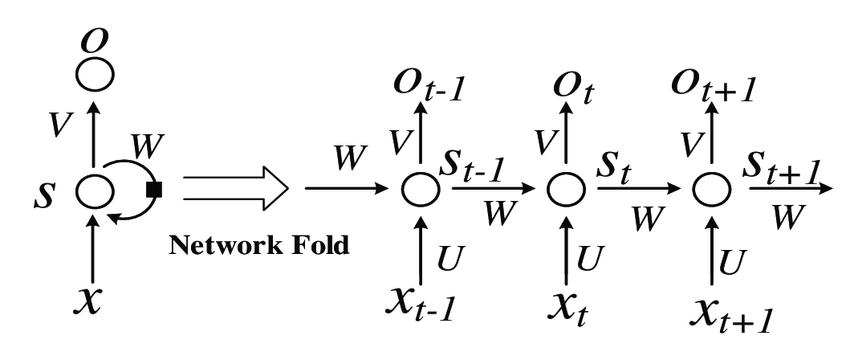
\includegraphics[scale=0.4]{images/literature review/RNN.png}
    \caption{Recurrent Neural Network architecture}
    \label{fig:ANN}
    \parencite{Gao2018}
\end{figure}
Recurrent neural network (RNN) are a category of artificial neural network optimized for sequential data processing \parencite{Jain1999}. This makes them particularly suitable for tasks involving time-series data, such as speech recognition, natural language processing, or time series prediction.

RNNs achieve their sequential data processing capability by incorporating loops within the network, allowing information to persist from one step in the sequence to the next. This 'memory' feature is what distinguishes RNNs from other neural network types, enabling them to effectively handle tasks that require understanding of context or the progression of inputs over time.

One of the most common architectures of RNN is the Long Short-Term Memory network. LSTM overcome one of the key limitations of standard RNNs, which is the difficulty in learning long-range dependencies due to vanishing or exploding gradients \parencite{DiPietro2020}. By incorporating a gating mechanism, LSTMs can selectively remember or forget information, making them more efficient at processing sequences where context from much earlier steps is important.

Despite their strengths, RNNs also present certain challenges. Training RNNs is difficult on 'chaotic' data as exploding and vanishing gradients keep occuring, which limits the expressivity of the RNN \parencite{Mikhaeil2021OnTD}. They can be computationally intensive and require careful optimization to prevent overfitting. Furthermore, while LSTMs address the vanishing gradient problem, they can still be complex to train effectively, and their inner workings can be hard to interpret.\\